\documentclass[a4paper,11pt, twoside]{article}

\usepackage[a4paper,top=3cm,bottom=3.5cm,left=2.5cm,right=2.5cm]{geometry}
\usepackage{graphicx}
\usepackage[utf8x]{inputenc}
\usepackage[italian]{babel}
\usepackage{fancyhdr}
\usepackage{amssymb}
\usepackage{makeidx}
\usepackage{hyperref}
\usepackage{varioref}
\usepackage{xmpincl}
\usepackage{ccicons}
\usepackage{subfigure}
\usepackage{listings}
\usepackage{color}

\definecolor{codegreen}{rgb}{0,0.6,0}
\definecolor{codegray}{rgb}{0.5,0.5,0.5}
\definecolor{codepurple}{rgb}{0.58,0,0.82}

\lstset{basicstyle=\small\ttfamily,
	keywordstyle=\color{blue}\bfseries,
	commentstyle=\color{green},
	stringstyle=\color{red},
	showstringspaces=true,
	numbers=left,
	frame=single,
	columns=fullflexible,
	breaklines=true,
	float=tb,
	captionpos=b}

\newcommand{\lstname}{Listato}

\title{Appunti di Middleware Technologies}
\author{Matteo Gianello}
\date{\today}

\pdfinfo{%
  /Title    (Appunti di Middleware Technologies)
  /Author   (Matteo Gianello)
  /Creator  (Matteo Gianello)
  /Producer ()
  /Subject  ()
  /Keywords (Middleware Tecnologies IngInf Polimi)
}
\makeindex
\includexmp{licenza}
\begin{document}
\pagestyle{empty}
\thispagestyle{empty}
\maketitle
\vspace{5cm}
\begin{center}
Quest'opera è stata rilasciata con licenza Creative Commons Attribuzione - Non commerciale - Condividi allo stesso modo 4.0 Internazionale. Per leggere una copia della licenza visita il sito web \url{http://creativecommons.org/licenses/by-nc-sa/4.0/}. \ccbyncsa.
\end{center}
\newpage

\thispagestyle{plain}
\tableofcontents
\newpage

\pagestyle{plain}
\section{Processi}\label{capitolo4}
In questo capitolo vedremo come i processi giochino un ruolo fondamentale nei sistemi distribuiti. Il concetto di processo proviene dall'ambito dei sistemi operativi ed è definito come un programma in esecuzione.\\
Per organizzare efficacemente un sistema client-server è spesso necessario utilizzare tecniche di \emph{multithreading} in quanto questa tecnica permette ai client e ai server di essere costruiti in modo tale che la comunicazione e l'elaborazione locale siano sovrapposti ottenendo un alto livello di prestazione.
\subsection{Thread}
Anche se i processi costituiscono la base di tutti i sistemi, la loro granularità non è sufficiente a soddisfare i bisogni dei sistemi distribuiti. una gestione più fine, sotto forma di \textbf{thread}, rende più facile la costruzione di applicazioni distribuite e ottenere prestazione migliori.
\subsubsection{Introduzione ai threads}
Prima di capire che cos'è un thread e che ruolo esso gioca nella costruzione di applicazioni distribuite è utile capire che cos'è in realtà un processo e che ruolo ha con i thread.\\
Per eseguire un programma, un sistema operativo crea un certo numero di processi virtuali. Per tener traccia di questi processi il sistema operativo mantiene aggiornata una \textbf{tabella dei processi} contenente elementi che vanno dalla memorizzazione dei registri della CPU, alla mappe della memoria, alla lista dei file aperti alle informazioni sugli \emph{account} e così via.\\
Il sistema operativo fa si che processi indipendenti non possano in alcun modo influire sulla correttezza degli altri processi, ovvero, è reso trasparente il fatto che più processi possano condividere concorrentemente la stessa CPU e le altre risorse hardware. Questa concorrenza però è ottenuta ad un prezzo abbastanza alto; ogni volta che viene creato un processo il sistema operativo deve creare uno spazio degli indirizzi completamente indipendente. Allocare memoria può voler dire inizializzare segmenti di memoria azzerando segmenti dati, copiare il programma in un segmento di testo e preparando uno \emph{stack} per i dati temporanei. Altrettanto costoso è il passaggio tra un processo ed un altro a livello di CPU, in quanto oltre a salvare il contesto è necessario cambiare i registri ed invalidare la cache.\\
Come un processo un \emph{thread} esegue il suo pezzo di codice indipendentemente dagli altri threads. A differenza dei processi nei threads non si cerca di ottenere un alto grado di trasparenza, in quanto il fatto di cercare di mantenere la trasparenza fa degradare le prestazione; di conseguenza un sistema basato sui thread gestisce l'insieme minimo delle informazioni per gestire la CPU. Infatti, il \textbf{contesto di un thread} è spesso costituito solamente dal contesto della CPU e dalle informazioni per gestire il thread stesso come ad esempio lo stato dovuto al blocco di una variabile \emph{mutex}. \uppercase{è} quindi compito degli sviluppatori proteggere l'accesso ai dati tra i vari threads di un singolo processo.
\paragraph{Utilizzo dei thread nei sistemi non distribuiti}
Il vantaggio principale dell'utilizzo dei thread nei sistemi non distribuiti deriva dal fatto che in un processo  a singolo thread quando viene effettuata una chiamata di sistema bloccante l'intero processo viene messo in pausa. Come nel caso di un foglio elettronico dove più celle sono collegate tra loro; in questo caso quando l'utente modifica il valore di una cella anche altre celle vengono rielaborate, ma tale rielaborazione è impensabile in un sistema a singolo thread in quanto il processo resterebbe bloccato in attesa di input e non calcolerebbe il valore delle altre celle.\\
Un altro vantaggio del multithreading è la possibilità di sfruttare il parallelismo quando si esegue il programma su sistemi multiprocessore. Il multithreading è usato anche nelle grandi applicazioni, le quali solitamente sono sviluppate come un insieme di processi cooperanti; tale cooperazione è realizzata tramite meccanismi di comunicazione tra processi (\emph{IPC, interprocess comunication}), ma questi meccanismi solitamente richiedono molti cambi di contesto che ne rallentano notevolmente le prestazioni. Invece di usare i processi un'applicazione può essere costruita mediante l'utilizzo di threads e la comunicazione tra questi avviene mediante l'uso dei dati condivisi, ed il passaggio da un thread all'altro può essere eseguito a livello utente.
\paragraph{Implementazione dei thread}
I thread sono spesso forniti sotto forma di pacchetto contente le operazioni di creazione e distruzione dei threads sia le operazioni per la loro sincronizzazione come \emph{mutex} e \emph{condition}. Gli approcci per implementare un pacchetto di thread sono due. Il primo è costruire una libreria che viene eseguita completamente a livello utente, il secondo è lasciare che il kernel sia conscio dei threads e si occupi del loro scheduling.\\
Usare una libreria utente ha notevoli vantaggi, prima di tutto la creazione e la distruzione dei threads a livello utente è molto meno costosa in quanto il costo è dovuto solo all'allocazione della memoria per creare uno \emph{stack}. Inoltre il cambio di contesto a livello utente può essere fatto con poche istruzioni. L'inconveniente principale dei thread a livello utente però è che una chiamata bloccante di sistema bloccherà l'intero processo e quindi bloccherà tutti i thread del processo.\\
Questo problema può essere raggirato implementando i threads a livello del kernel ma questo comporta che ogni operazione eseguita su un thread (creazione, distruzione, sincronizzazione e così via) dovrà essere eseguita a livello del kernel richiedendo quindi una chiamata a sistema che risulta essere molto più lenta e costosa come quella di un processo.\\
La soluzione ai problemi sta nell'uso di una forma ibrida chiamata \textbf{processi lightweight}. Un processo leggero viene eseguito nel contesto di un singolo processo (pesante) e per ogni processo ci possono essere più processi leggeri. Oltre a questi il sistema fornisce un pacchetto a livello utente per i threads mettendo a disposizione le solite operazioni. Il pacchetto dei thread è condivisibile da tutti i processi leggeri; questo significa che ogni processo leggero può eseguire il suo thread. Le applicazioni multithread vengono costruite creando dei thread e successivamente assegnando questi thread a un processo leggero.\\
Il pacchetto dei thread ha una singola routine per pianificare il thread successivo. Quando si crea un processo leggero gli si assegna uno \emph{stack} e lo si mette alla ricerca di un thread da eseguire. I thread in esecuzione sono sono salvati in una tabella in una tabella alla quale i processi leggeri accedono in mutua esclusione tramite l'uso di \emph{mutex} nello spazio utente. Questo significa che la sincronizzazione tra threads è interamente eseguita a livello utente senza la necessità di informare il kernel. \\
Nel caso in cui vi sia una chiamata di sistema bloccante il contesto di esecuzione passa dalla modalità utente a quella kernel ma continua comunque nel contesto del processo leggero attuale. Nel momento in cui il processo leggero non può più proseguire allora il sistema può decidere di proseguire con un altro processo leggero ritornando alla modalità utente.\\
I vantaggi di utilizzare un sistema ibrido sono molti. Innanzitutto la creazione, la distruzione e la sincronizzazione dei threads è relativamente poco costosa in quanto avviene a livello utente. Se un processo ha abbastanza processi leggeri allora una chiamata bloccante di sistema non bloccherà l'intero processo. A livello di architetture multiprocessore processi leggeri diversi possono essere eseguiti su CPU diverse.
L'unico inconveniente che si presenta è che i processi leggeri devono essere creati e distrutti ma fortunatamente tali operazioni non sono comuni.
\subsubsection{Thread nei sistemi distribuiti}
Come abbiamo visto il vantaggio principale dell'uso dei threads è che una chiamata di sistema bloccante non blocca l'intero processo. Questa caratteristica è molto vantaggiosa nel caso di realizzazione di comunicazioni multiple come ad esempio la gestione di comunicazioni client-server.
\paragraph{Client multithread}
Per raggiungere un buon grado di trasparenza alla distribuzione i sistemi distribuiti che operano su reti globali hanno la necessità di nascondere lunghi tempi di propagazione dei messaggi. La tecnica più comune per nascondere la latenza dei messaggi è quella di avviare la comunicazione ed immediatamente iniziare a fare qualcos'altro.
Un esempio molto diffuso sono i browser web che iniziano la comunicazione, ricevono una parte del codice HTML ed iniziano a visualizzare la pagina prima ancora di aver concluso la comunicazione.
\paragraph{Server multithread}
Anche se l'uso di client multithread offre notevoli vantaggi, il vero uso del multithreading è lato server. La pratica dimostra come l'uso del multithreading semplifica la codice e rende più facile lo sviluppo di applicazioni parallele per ottenere un alto livello di prestazioni.\\
Vediamo il caso di un \emph{file server} dove un \textbf{dispacher} riceve in ingresso su di una porta le richieste provenienti da diversi client. Dopo averla esaminata il dispacher seleziona un \textbf{worker thread} inattivo a cui assegnare la richiesta. Il \emph{worker} procede con la richiesta ed esegue una lettura bloccante sul file system locale; questo può far si che il thread vengo bloccato in attesa della lettura da disco, in tal caso viene selezionato un altro thread (\emph{worker} o \emph{dispacher}) che procede con la sua esecuzione.
\subsubsection{Il modello preemtive}
Nei sistemi moderni oltre ai thread viene utilizzato il modello \emph{preemtive}, ovvero è possibile forzare un processo ad abbandonare il suo stato di esecuzione. Solitamente questo meccanismo è utilizzato per implementare un meccanismo di \emph{time slicing} come mostrato in \figurename~\ref{fig:preemtive}.
\begin{figure}
\centering
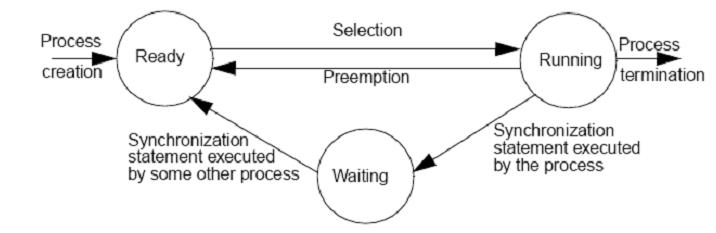
\includegraphics[scale=0.8]{img/preemtive.png}
\caption{Modello preemtive}\label{fig:preemtive}
\end{figure}
\subsection{I thread in C}
Tutti i sistemi UNIX sono multitasking con il sistema preemptive; tradizionalmente tutti i processi sono creati allo stesso modo tramite l'uso della primitiva \texttt{fork()}. La \emph{fork}produce una copia del processo chiamante; questa copia è esattamente identica all'origina tranne per il valore restituito dalla \texttt{fork} che per il processo figlio vale \emph{0} mentre nel padre il valore restituito è il \emph{pid} del figlio. Un piccolo esempio:
\begin{lstlisting}[language=C,float=htb,captionpos=b,caption={Esempio di uso della fork},label=lst:fork]
/*do parent stuff*/
ppid = fork ();
if (ppid < 0) {
	fork_error_function ();
} else if (ppid == 0) {
	child_function ();
} else {
	parent_function ();
}
\end{lstlisting}
La fork restituisce due copie completamente indipendenti dello stesso processo, questa indipendenza permette la protezione della memoria e la stabilità ma causa dei problemi quando si vuole che diversi processi lavorino sullo stesso problema; infatti sarebbe necessario usare \emph{pipes} oppure \emph{SysV IPC}. Inoltre il costo di switching tra processi multipli è molto alto, la sincronizzazione è lenta ed esistono dei limiti sul numero di processi che possono essere schedulati efficacemente.\\
Per questo sono stati introdotti i threads che invece possono essere schedulati all'interno del processo e risolvono molti problemi del lavoro multi processo.
L'API più popolare per creare una applicazione multithread in ambiente UNIX è la \emph{pthread} (\emph{POSIX thread}).\\
Le operazioni che si possono eseguire con quest'API sono la creazione, la distruzione, la sincronizzazione (\emph{join}), lo scheduling, il controllo dei dati e l'interazione con il processo principale. I threads dello stesso processo condividono le istruzioni di processo, gran parte dei dati, i descrittori dei file aperti, i segnali e lo user e il group id. Mentre per ogni thread abbiamo un distinto \emph{ThreadID}, un certo numero di registri, uno stack pointer ed una certa priorità come possiamo vedere \figurename~\ref{fig:threadstack}.
\begin{figure}[hbt]
\subfigure[]{
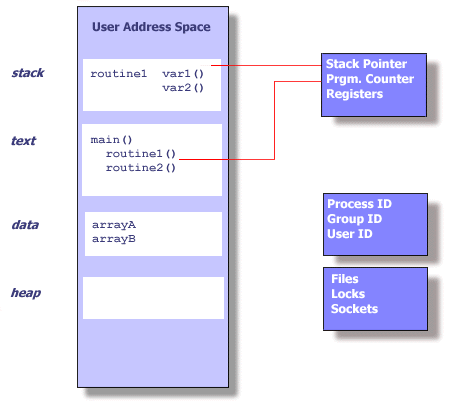
\includegraphics[width=7.5cm]{img/stack.png}
\label{fig:stack}
}
\subfigure[]{
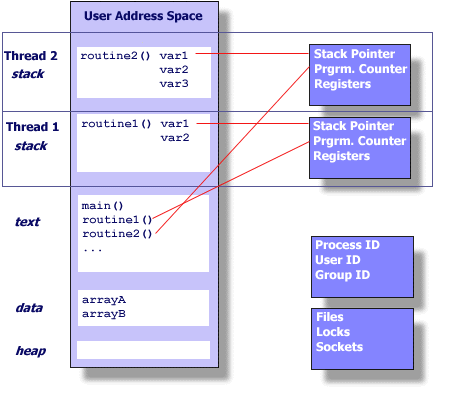
\includegraphics[width=7.5cm]{img/threadstack.png}
\label{fig:stackthread}
}
\caption{Memoria nel caso di processo (a) e di thread (b)}\label{fig:threadstack}
\end{figure}
Vediamo ora quali sono le funzioni della API \emph{pthread}
\paragraph{Thread creation}
La funzione per la creazione dei thread è:
\begin{lstlisting}[language=C,float=htb,captionpos=b,caption={Funzione di creazione dei thread},label=lst:creation]
int pthread_create (pthread_t *id, const pthread_attr_t *attr, void *(*routine)(void *), void *arg)
\end{lstlisting}
dove i valori sono:
\begin{description}
\item[id:] un valore che identifica il thread che viene restituito dalla funzione.
\item[attr]: un attributo che può essere utilizzato per impostare alcuni valori del thread. Se viene impostato a \emph{NULL} vengono impostati i valori di default.
\item[routine:] indica la funzione C che il thread eseguirà una volta creato.
\item[arg:] un singolo argomento che può essere passato a\texttt{routine}, deve essere passato come riferimento ad un puntatore di tipo \texttt{void}; in caso non vi siano valori si imposta a \emph{NULL}.
\end{description}
\paragraph{Thread termination}
Esistono diversi modi in cui un pthread può terminare:
\begin{itemize}
\item Il thread termina la sua routine.
\item Nel thread viene richiamata la \texttt{pthread\_exit}.
\item Il thread è cancellato da un altro thread tramite la chiamata della funzione \texttt{pthread\_cancel}.
\item L'intero processo termina quando viene chiamata una delle funzioni \texttt{exec} o \texttt{exit}.
\end{itemize}
Tramite la \texttt{pthread\_exit} è possibile specificare uno stato di terminazione che può essere restituito alla sincronizzazione del thread. Inoltre è molto importante ricordare che la \texttt{pthread\_exit} non chiude i file ed ogni file aperto all'interno del thread rimane aperto anche alla sua terminazione.
Se la funzione \emph{main} termina con una \texttt{pthread\_exit} prima che i threads siano conclusi i threads proseguono la loro esecuzione altrimenti terminano alla conclusione del \emph{main}.
Vediamo un esempio di creazione e terminazione dei thread in C nel Listato \ref{lst:thread}
\lstinputlisting[language=C,caption={Esempio di uso della API pthread},label=lst:thread]{listati/ThreadExample1.c}
\paragraph{Passaggio di argomenti}
Come abbiamo visto nella \emph{pthread\_create} è possibile impostare l'ultimo attributo con un attributo da passare alla routine che il thread eseguirà. Tale attributo deve essere convertito in un puntatore di tipo void. Tale passaggio presenta però alcuni tranelli, vediamo come nel Listato \ref{lst:wrongpass} come il passaggio per indirizzo crei un errore nell'esecuzione. Infatti, provando ad eseguire tale programma si rischia che più di un thread acceda contemporaneamente alla variabile \emph{t} e si rischiano quindi di ottenere dei valori sbagliati.
\begin{lstlisting}[language=C,caption={Errore nel passaggio di argomenti ad un thread},label=lst:wrongpass]
int rc, t;
for(t=0; t<NUM_THREADS; t++) {
	printf("Creating thread %d\n", t);
	rc = pthread_create(&threads[t], NULL, PrintHello, (void *) &t);
	...
}
\end{lstlisting}
Un possibile risultato di questo codice è quello seguente dove si può vedere che il thread numero 3 stampa il valore 4 anche se il thread numero 4 non è ancora stato creato (In realtà tutti i thread accedono alla variabile \emph{t} con un ritardo in quanto manca la stampa del thread numero 0).
\begin{verbatim}
Creazione del thread 0
Creazione del thread 1
1: Hello World!
Creazione del thread 2
2: Hello World!
Creazione del thread 3
3: Hello World!
4: Hello World!
Creazione del thread 4
\end{verbatim}
Per passare un argomento ad una routine è necessario controllare l'accesso ai dati da parte dei threads in modo che non vi siano possibili conflitti come nel caso del Listato \ref{lst:rightpass}. Nel quale viene passato ad ogni routine un puntatore ad un dato diverso.
\begin{lstlisting}[language=C,caption={Metodo corretto nel passaggio di argomenti ad un thread},label=lst:rightpass]
int *taskids[NUM_THREADS];
for(t=0; t<NUM_THREADS; t++) {
	taskids[t] = (int *) malloc(sizeof(int));
	*taskids[t] = t;
	printf("Creating thread %d\n", t);
	rc = pthread_create(&threads[t], NULL, PrintHello, (void *) taskids[t]);
	...
}
\end{lstlisting}
\paragraph{Joining threads}
L'operazione di \emph{join} è uno dei modi nel quale si può implementare la sincronizzazione tra thread.
\begin{lstlisting}[language=C]
int pthread_join(pthread_t thid,void **thread_return)
\end{lstlisting}
dove i diversi campi sono:
\begin{description}
\item[thid] è l'identificativo del thread su cui fare la join
\item[thread\_return] è il possibile valore di ritorno che si ottiene dall'invocazione della \texttt{pthread\_exit}
\end{description}
Il funzionamento della funzione di \emph{join} è specificato in \figurename\, \ref{fig:join}
\begin{figure}[htb]
\centering
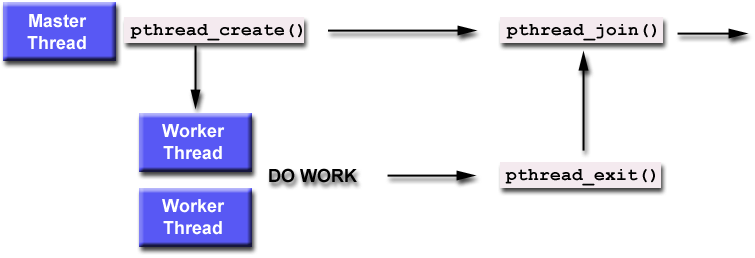
\includegraphics[scale=0.7]{img/join.png}
\caption{Funzionamento dell'operazione di join}\label{fig:join}
\end{figure}
\paragraph{I mutex}
Un \emph{mutex} funziona come un \emph{lock} proteggendo l'accesso a dei dati condivisi. Il concetto principale è che un solo thread alla volta può bloccare una variabile di tipo mutex, se più thread tenta di bloccare un mutex soltanto uno di questi effettuerà l'operazione con successo, inoltre i thread non possono bloccare un determinato mutex finché il thread che lo detiene non lo libera.\\
\uppercase{è} compito del programmatore assicurarsi che ogni thread che utilizza dei dati condivisi usi i mutex.\\
Una variabile di tipo mutex può essere dichiarata sfruttando la parola chiave \texttt{pthread\_mutex\_t}, per inizializzare tale variabile, invece, è possibile sfruttare due metodi:
\begin{itemize}
\item Il primo è l'inizializzazione statica come ad esempio
\begin{verbatim}
pthread_mutex_t mymutx = PTHREAD_MUTEX_INITIALIZER;
\end{verbatim}
\item Il secondo metodo è l'inizializzazione dinamica richiamando la routine
\begin{verbatim}
pthread_mutex_init
\end{verbatim}
In questo caso è possibile impostare alcuni parametri dell'oggetto mutex tramite le primitive \texttt{pthread\_mutexattr\_init} e \texttt{pthread\_mutexattr\_destroy} che rispettivamente creano e distruggono gli attributi  di un mutex
\end{itemize}
In entrambi i casi di inizializzazione l'oggetto mutex è inizializzato \emph{unlocked}. Infine, la routine \texttt{pthread\_mutex\_destroy} permette di rilasciare un mutex di cui non si ha più bisogno.\\
Esistono tre primitive per la gestione dei mutex, queste sono:
\begin{itemize}
\item \texttt{pthread\_mutex\_lock:} che si usa per acquisire un lock su di una variabile, nel caso in cui tale lock sia detenuto da un altro thread il thread che ha richiesto il lock si blocca finché il blocco non viene rilasciato.
\item \texttt{pthread\_mutex\_trylock} molto simile alla routine precedente solo che nel caso in cui il blocco sia detenuto da un altro thread allora la routine restituisce un codice di errore che indica \emph{"busy"}; è molto utile nel caso si vogliano prevenire condizioni di deadlock.
\item \texttt{pthread\_mutex\_unlock:} questa routine permette di rilasciare il lock in possesso del thread ma restituisce un errore nel caso in cui si voglia rilasciare un lock su di una variabile già sbloccata o bloccata da un altro thread.
\end{itemize}
\lstinputlisting[language=C,caption={Esempio di uso delle variabili mutex},label=lst:mutex]{listati/ThreadExample2.c}
\paragraph{Condition variables}
Mentre i mutex implementano la sincronizzazione tramite il controllo degli accessi sui dati le \emph{condition variables} permettono ai thread di sincronizzarsi in base ad un determinato valore di un dato. Senza quest'aspetto dei thread bisognerebbe implementare un polling per verificare quando una particolare condizione viene riscontrata. Le \emph{condition variables} sono un modo per ottenere lo stesso risultato senza il polling, e possono essere utilizzate anche insieme ai mutex.
L'utilizzo principale sono tutti quei problemi della categoria\textbf{produttore-consumatore}.\\
Come per i mutex le condition variabile sono dichiarate utilizzando la parola chiave \texttt{pthread\_cond\_t}; per l'inizializzazione esistono due metodi:
\begin{itemize}
\item Statico
\begin{verbatim}
pthread_cond_t myconvar = PTHREAD_COND_INITIALIZER
\end{verbatim}
\item Dinamico tramite la funzione \texttt{pthread\_cond\_init} che permette di settare anche gli attributi della variabile tramite le due primitive
\begin{verbatim}
pthread_condattr_init
pthread_condattr_destroy
\end{verbatim}
Che permettono rispettivamente di inizializzare e distruggere gli attributi della variabile
\end{itemize}
Infine tramite la primitiva \texttt{pthread\_cond\_destroy} è possibile liberare una variabile condizionale che non è più necessaria.\\
Per la gestione di questo tipo di variabile esistono diverse primitive:
\begin{itemize}
\item \texttt{pthread\_cond\_wait} è una routine che il thread finché una determinata condizione non si verifica, se chiamata quando vi è un lock attivo la routine sblocca il mutex e lo blocca nuovamente quando il thread si sveglia.
\item \texttt{pthread\_cond\_signal} questa routine risveglia gli altri thread in attesa di una \emph{condition variables}
\item \texttt{pthread\_cond\_brodcast} può essere utilizzata al posto della routine precedente se ci sono più thread bloccati in uno stato di \emph{"wait"}.
\end{itemize}
\subsection{Concorrenza in Java}
Come per il C anche il Java fornisce il supporto alla concorrenza a livello di linguaggio, esso mette a disposizione delle classi per istanziare ed eseguire nuovi thread più i metodi di sincronizzazione e le variabili di condizione.
Il modo più semplice per creare un thread è quello di utilizzare la classe \texttt{java.lang.Thread} in questo caso è sempre necessario implementare un metodo \texttt{run()}.
\begin{lstlisting}[language=Java,caption={Uso della classe Thread in Java},label=lst:jthread]
public class MyThread extends Thread {
	private String message;
	public MyThread(String m) {message = m;}
	public void run() {
		for(int r=0; r<20; r++)
			System.out.println(message);
	}
}

public class ProvaThread {
	public static void main(String[] args) {
		MyThread t1,t2;
		t1=new MyThread("primo thread");
		t2=new MyThread("secondo thread");
		t1.start();
		t2.start();
	}
}
\end{lstlisting}
Come vediamo la nostra classe che implementa un thread estende l'oggetto \emph{Thread}, in questa classe viene fatto l'override del metodo \texttt{run()} il quale non è altro che la routine che viene eseguita dal thread. Per far partire il thread è necessario richiamare il metodo \texttt{start()} dopo aver creato un nuovo oggetto.\\
Un'altra possibile soluzione è l'utilizzo dell'interfaccia \texttt{Runnable} la quale specifica soltanto che deve esistere un metodo \texttt{run()} che deve essere implementato. La classe \texttt{Thread} implementa anch'essa l'interfaccia \texttt{Runnable}.
Come vediamo nel Listato\,\ref{lst:runnable} a differenza del caso precedente oltre all'oggetto \emph{MyThread} deve anche essere creato un oggetto \emph{Thread} corrispondente, al quale viene poi passato l'oggetto MyThread, ed infine il metodo \texttt{start()}viene invocato sull'oggetto Thread.
\lstinputlisting[language=Java,caption={Utilizzo dell'interfaccia Runnable},label=lst:runnable]{listati/MyThread.java}
L'esecuzione dei thread non segue un ordine predefinito ma lo stesso codice può produrre risultati diversi su diversi computer o addirittura sullo stesso. Questo caratteristica è chiamata \emph{non-determinismo} ed è un punto focale nella concorrenza.\\
Java di per se implementa il modello \emph{preemtive} e nel caso sia disponibile un meccanismo di \emph{time-slicing} allora java esegue i thread con la stessa priorità tramite una meccanismo di \emph{round-robin}.\\
Per definire quando un sistema multithread è corretto si devono rispettare due proprietà:
\begin{itemize}
\item\emph{Sicurezza:} Un sistema si dice sicuro quando gli eventi malevoli non accadono.
\item\emph{Longevità:} Un sistema è longevo quando le cose buone possono accadere.
\end{itemize}
I possibili guasti che rientrano nella categoria "Sicurezza" sono quei guasti che avvengono a livello di esecuzione come i conflitti \emph{read/write} e \emph{write/write}. I meccanismi che invece riguardano la "Longevità" sono quei meccanismi che bloccano l'esecuzione del programma come:
\begin{itemize}
\item Lock
\item Waiting
\item CPU contention
\end{itemize}
Solitamente, purtroppo, le cose più semplici che si possono fare per aumentare la longevità ne riducono però la sicurezza e vice versa.\\
Vediamo ora quali sono i meccanismi che Java mette a disposizione per supportare la concorrenza.
\paragraph{Exclusion}
In un sistema sicuro ogni oggetto protegge se stesso da possibili violazioni della sua integrità. le tecniche di esclusione preservano l'invariante di un oggetto. Tre sono le tecniche principali per permettere l'\emph{esclusione}:
\begin{itemize}
\item Immutabilità
\item Esclusione dinamica (Locking)
\item Esclusione strutturale
\end{itemize}
Per quanto riguarda l'\textbf{immutabilità} si ottiene creando le classi in modo che gli oggetti proteggano se stessi come nel Listato\,\ref{lst:immutabile}
\begin{lstlisting}[language=Java,caption={Esempio di oggetto immutabile},label=lst:immutabile]
class ImmutableAdder {
	private final int offset;
	public Immutableadder (int a) {
		offset = a;
	}
	public int addOffset (int b) {
		return offset + b;
	}
}
\end{lstlisting}
I vantaggi di questa tecnica sono il fatto che non richiede sincronizzazione ed è molto utile per condividere degli oggetti tra i threads, ma sfortunatamente ha dei limiti di applicabilità.\\
Per parlare di sincronizzazione introduciamo prima l'esempio del Listato\,\ref{lst:sincro}
\begin{lstlisting}[language=Java,caption={Esempio sincronizzazione},label=lst:sincro]
public class RGBColor {
	private int r;
	private int g;
	private int b;
	
	public void setColor (int r, int g, int b)
		checkRGBVals(r, g, b);
		this.r = r;
		this.g = g;
		this.b = b;
	}
}
\end{lstlisting}
Ora immaginiamo che due thread chiamati \emph{red} e \emph{blue} vogliano impostare contemporaneamente il loro colore sullo stesso oggetto di tipo \texttt{RGBColor} a questo punto potrebbero verificarsi dei problemi in quanto i due thread tentano di scrivere lo stesso dato violando così la sua integrità.\\
Per risolvere questo problema java tramite il locking serializza l'esecuzione del codice dichiarato \emph{synchronized}. Ogni istanza di un oggetto possiede tali meccanismi di lock in quanto derivati dalla classe \texttt{Object}, l'unica eccezione si ha con l'utilizzo di array, infatti, bloccare un array non blocca gli elementi di tale array.\\
Esistono due modi per bloccare una parte di codice, si può dichiarare \emph{synchronized} un intero metodo o un singolo blocco di codice, in caso di singolo blocco la funzione \texttt{synchronized} richiede l'oggetto sul quale effettuare il lock (Listato\,\ref{lst:syncobj} e Listato\,\ref{lst:syncmeto}).\\
\pagebreak
\begin{lstlisting}[language=Java,caption={Sincronizzazione di una parte di codice},label=lst:syncobj]
synchronized (object) {
	//Lock is held
	...
}
//Lock is released
\end{lstlisting}
\begin{lstlisting}[language=Java,caption={Sincronizzazione di un metodo},label=lst:syncmeto]
synchronized void f() {
	//Lock is held
	/* Body */
}
//Lock is released
\end{lstlisting}
I lock vengono automaticamente acquisiti all'ingresso del blocco o del metodo dichiarato \texttt{synchronized} e rilasciato all'uscita da esso.\\
Alcune regole chiave per l'uso della sincronizzazione sono:
\begin{itemize}
\item Sempre quando si effettua un aggiornamento a dei campi di un oggetto.
\begin{lstlisting}[language=Java]
synchronized (point) {
	point.x = 5; point.y = 7;
}
\end{lstlisting}
\item Tutte le volte che si accede a dei dati che potrebbero essere aggiornati.
\begin{lstlisting}[language=Java]
synchronized (point) {
	if (point.x > 0) {...}
}
\end{lstlisting}
\item Si può fare a meno di sincronizzare parti di metodo stateless
\begin{lstlisting}[language=Java]
public void f() {
	synchronized (this) {
		state = ...;
	}
	operations();
}
\end{lstlisting}
\item \textbf{Mai} sincronizzare parti di codice che contengono invocazioni ad altri oggetti
\begin{lstlisting}[language=Java]
public void f() {
	synchronized (this) {
		...
	}
	h.foo();
}
\end{lstlisting}
\end{itemize}
La strategia più sicura (ma non la più efficace) per realizzare un'applicazione OO concorrente è quella di utilizzare oggetti completamente sincronizzati, anche detti oggetti \emph{atomici}, nei quali tutti i metodi sono sincronizzati, non esistono campi pubblici o altri tipi di violazione nell'incapsulamento, tutti i metodi sono finiti e hanno modo di rilasciare il lock, tutti i campi sono inizializzati ad un valore consistente nel costruttore, ed infine lo stato dell'oggetto è consistente sia all'inizio che alla fine di ogni metodo anche in presenza di eccezioni.\\
Uno dei problemi principali della programmazione concorrente è il \emph{deadlock}, tale problema si verifica quando due o più oggetti sono acceduti da due o più threads e tali thread detengono un lock mentre tentano di acquisire un lock detenuto da un altro thread.\\
L'assegnamento di un valore ad una variabile è un'operazione atomica (a parte per i \emph{long} e i \emph{double}), questo significa che generalmente non è necessario sincronizzare l'accesso ad una variabile. Tuttavia i thread solitamente memorizzano il valori delle variabile in memoria locale, questo significa che se un thread cambia il valore di una variabile un altro thread non vede il cambiamento. Per evitare questo meccanismo bisogna sincronizzare la variabile oppure dichiararla di tipo \texttt{volatile} che significa che ogni volta che una variabile è usata deve prima essere letta dalla memoria principale.\\
Il confinamento implementa l'incapsulamento garantendo che al massimo un'attività alla volta acceda agli oggetti. Questo meccanismo permette l'accesso ad un solo thread alla volta senza utilizzare i locking dinamici.
Il punto principale è quello avere un punto di uscita dal thread. Esistono quattro categorie per verificare che un riferimento \emph{r} ad un oggetto \emph{x} può uscire da un metodo \emph{m}:
\begin{itemize}
\item \emph{m} passa \emph{r} come argomento di un'invocazione ad un metodo o ad un costruttore di un oggetto
\item \emph{m} passa \emph{r} come valore di ritorno di un metodo.
\item \emph{m} registra \emph{r} in un campo accessibile da altre attività
\item \emph{m} rilascia un riferimento che però permette l'accesso ad \emph{r}
\end{itemize}
Per quanto riguarda le collezioni, il framework \texttt{java.util.Collection}  basata su uno schema \emph{Adapter} permette la sincronizzazioni delle classi collection, infatti, ad eccezione di \texttt{Vector} e \texttt{Hashtable} le classi base per le collezioni (come \texttt{java.utili.ArrayList}) sono non sincronizzate. Sono state così costruite una serie di classi sincronizzate attorno alle classi base come la \texttt{Collection.synchronizedList}.\\
Come abbiamo detto prima però la sincronizzazione non è molto efficiente infatti richiamare un metodo sincronizzato richiede un tempo quattro volte maggiore rispetto a metodi non sincronizzati; inoltre, esso riduce la concorrenza e diminuisce le performance, infine non vi è alcun modo di controllare il meccanismo dei lock.\\
Con java versione 5 sono stati introdotti nuovi meccanismi di sincronizzazione come la \emph{sincronizzazione condizionata.} Prendiamo come esempio un parcheggio con una certa capacità e dei metodi che permettono l'arrivo e la partenza di automobili come esemplificato nel Listato\,\ref{lst:monitor}.
\begin{lstlisting} [language=Java,caption={Esempio di controllore di un parcheggio},label=lst:monitor]
public class CarParkControl {
	protected int space;
	protected int capacity;
	
	public CarParckControl (int n) {
		capacity = space = n;
	}
	
	syncronized public void arrive() {
		...; --space; ...;
	}
	syncronized public void depart() {
		...; ++space; ...;
	}
}
\end{lstlisting}
Come per il C esistono però dei metodi che permettono una gestione più efficiente del controllore rispetto all'uso della syncronized; questi metodi sono:
\begin{itemize}
\item \texttt{public final void notify()}: che risveglia un singolo thread in attesa.
\item \texttt{public final void notifyAll()}: risveglia tutti i thread in attesa.
\item \texttt{public final void wait() throws InterruptedException}: pone il thread in attesa di un \emph{notify}. Quando un thread viene posto in uno stato di wait esso rilascia il lock acquisito e lo riacquista al suo risveglio.
\end{itemize}
\lstinputlisting[language=Java,caption={Esempio di variabili condizionali in Java},label=lst:jsincro]{listati/CarParkControl.java}
Si può ridurre l'overhead dovuto al contex-switching sostituendo la \texttt{notifyAll} con la \texttt{notify}. Tale meccanismo può essere usato per migliorare le performance quando si è certi che almeno un thread è in atteso per eseguire un lavoro.\\
Alla condizione di \emph{wait} è possibile associare un timer molto utile per migliorare la longevità del sistema in quanto tende a risolvere in modo automatico i deadlock.
\section{Core Comunication Facilities}
\subsection{Socket}
Nella programmazione di rete esistono diversi tipi di protocolli tra cui l'\emph{unicast TCP}, l'\emph{unicast UDP} e il \emph{multicast IP}. Per ogni protocollo esiste un RFC che descrive come questi protocolli lavorano in pratica, tuttavia, il problema principale è capire come un programmatore possa trarre vantaggio da questi protocolli. La risposta a questa domanda sono i \textbf{Socket}, comparsi per la prima volta 1982 nel sistema Unix BSD oggi sono disponibili per qualsiasi sistema. I \emph{socket} forniscono un'astrazione comune per la comunicazione interprocesso sia essa di tipo \emph{connection-oriented (TCP)} sia di tipo \emph{connection-less (UDP)}.\\
\subsubsection{I socket in C}
Il flusso di esecuzione di una comunicazione tra due processi segue lo schema in \figurename"\ref{fig:streamsocket} in questo caso si tratta di una comunicazione orientata alla connessione infatti vediamo come il processo \emph{client} (quello a destra) effettui una \texttt{connect()} prima di inviare o ricevere dei dati.
\begin{figure}
\centering
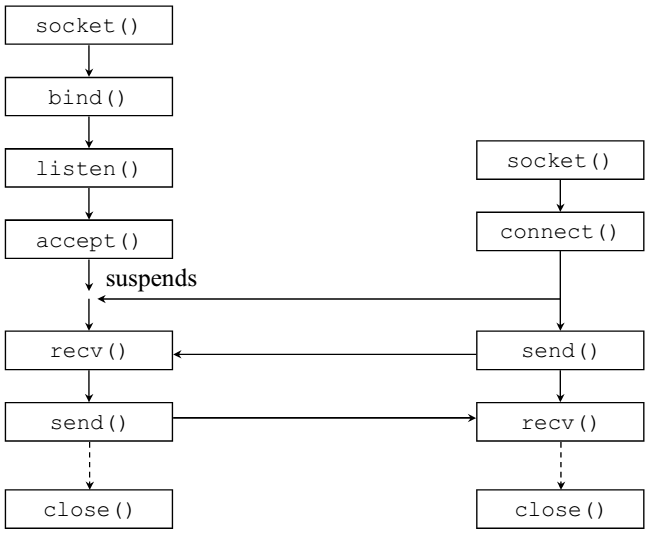
\includegraphics[width=0.7\linewidth]{img/streamsocket}
\caption{Flusso di esecuzione di una comunicazione orientata alla connessione}
\label{fig:streamsocket}
\end{figure}
Vediamo ora due esempi di un client e di un server TCP rispettivamente nel Listato \ref{lst:clienttcp} e nel Listao \ref{lst:servertcp}
\lstinputlisting[language=C,caption={Client TCP},label=lst:clienttcp]{listati/ClientTCP.c}
\lstinputlisting[language=C,caption={Server TCP},label=lst:servertcp]{listati/ServerTCP.c}
Abbiamo visto come funziona una comunicazione orientata alla connessione vediamo ora come funziona invece una comunicazione di tipo \emph{connection-less} mostrata in \figurename"\ref{fig:udpcon}.
\begin{figure}
\centering
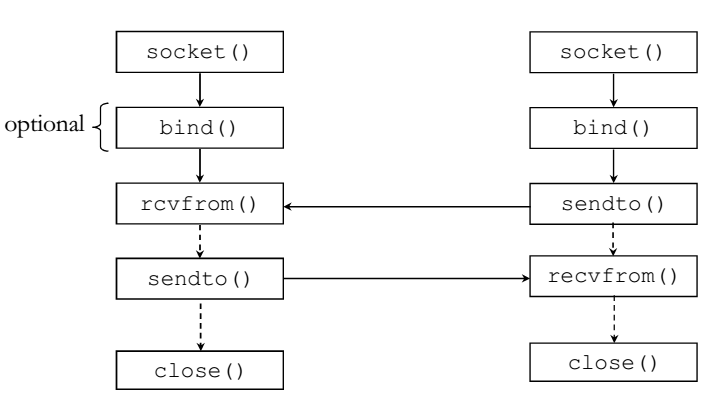
\includegraphics[width=0.7\linewidth]{img/udpcon}
\caption{Flusso di esecuzione di una comunicazione senza connessione}
\label{fig:udpcon}
\end{figure}
Come vediamo in questo caso non è necessario effettuare l'\texttt{accept} ne la \texttt{connect} in quanto i messaggi sono inviati direttamente, questo meccanismo è più rapido del precedente ma risulta essere meno sicuro.
\subsubsection{I socket in Java}
In Java l'approccio ai \emph{socket} è simile al C risulta tuttavia molto più semplice. Esistono cique classi principali fornite dal \emph{package} \texttt{java.net} queste classi sono:
\begin{itemize}
\item \texttt{InetAddress:} fornisce i metodi per ottentere l'indirizzo di un host dato il suo \emph{hostname} e vice versa
\item \texttt{ServerSocket:} utilizzata dal server per accettare le connessioni in ingresso.
\item \texttt{Socket:} la classe principale utilizzata per la comunicazione
\item \texttt{DatagramPacket:} classe utilizzata per inviare messaggi attraverso un  \texttt{DatagramSocket}
\item \texttt{DatagramSocket:} classe utilizzata per l'invio e la ricezione di messaggi senza l'ausilio di una connessione
\end{itemize}
Un esempio di un client e di un server TCP in Java è mostrato rispettivamente nel Listato \ref{lst:javaclient} e nel Listato \ref{lst:javaserver}.
Vediamo come in java la comunicazione avvenga tramite input e output stream associati ad una socket.
\lstinputlisting[language=Java,caption={Client TCP in Java},label=lst:javaclient]{listati/TCPClient.java}
\lstinputlisting[language=Java,caption={Server TCP in Java},label=lst:javaserver]{listati/TCPServer.java}
Le classi \texttt{ObjectInputStream} e \texttt{ObjectOutputStream} permettono di leggere e scrivere su di uno stream serializzato; per essere trasmesso su questo tipo di stream un oggetto deve essere serializzabile ovvero deve implementare l'interfaccia \texttt{Serializable}. La serializzazione permette una \emph{copia profonda} di un oggetto. Un programmatore può impedire la serializzazione di un oggetto dichiarandolo di tipo \texttt{transient}.
\subsubsection{IP Multicast}
Il \textbf{multicast IP} è un protocollo di rete che permette la consegna di pacchetti UDP a molti destinatari contemporaneamente. Per implementare tale protocollo solitamente si riservano degli indirizzi IP di classe D per i gruppi \emph{multicast}.\\
I componenti interessati a ricevere dei messaggi inviati in un gruppo devono effettuare una \emph{join} a tale gruppo, non è necessario, invece, unirsi al gruppo per inviare un messaggio indirizzato ad un determinato gruppo.\\
Java fornisce una sottoclasse della classe \texttt{DatagramSocket} denominata \texttt{MulticastSocket} per implementare in modo semplice il multicast; questa classe aggiunge due metodi alla classe \texttt{DatagramSocket} che sono il \texttt{joinGroup} e il \texttt{leaveGroup}.
\subsection{Remote procedure call}
Con lo sviluppo della programmazione il problema che si è presentato è che l'interazione tra client e server avveniva sempre tramite le primitive di I/O del sistema, questo rendeva le applicazioni difficili da sviluppare. L'idea di \emph{Sun Microsystems} è stata quella di permettere l'accesso remoto attraverso un meccanismo ben conosciuto ovvero quello delle chiamate a procedura come mostrato in \figurename \ref{fig:rpc}.
\begin{figure}[tb]
\centering
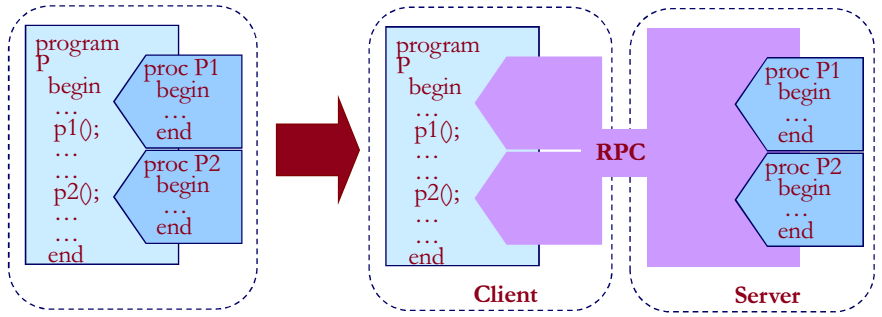
\includegraphics[width=0.7\linewidth]{img/rpc}
\caption{Modello di chiamata a procedura remota}
\label{fig:rpc}
\end{figure}
Tuttavia questo modello comporta alcuni problemi soprattutto per quanto riguarda il passaggio dei parametri. Il primo problema dovuto al passaggio dei parametri è quello della conversione di strutture dati complesse come oggetti o \texttt{struct} in uno stream di byte sequenziale, tale problema è chiamato \emph{serializzazione}. Il secondo problema che si presenta è il fatto che un sistema host potrebbe usare una rappresentazione dei dati differente ed è quindi necessaria una conversione, tale problema è chiamato \emph{marshalling}.\\
I middleware forniscono supporto automatico per risolvere questi problemi, il marshaling e la serializzazione sono implementati automaticamente e entrano a far parte dello stub; inoltre permettono un'indipendenza dal linguaggio in quanto le procedure vengono rappresentate tramite un \emph{Interface Definition Language} (IDL).\\
L'\emph{interface definition language} alza il livello di astrazione della definizione del servizio separando l'\emph{interfaccia} del servizio dalla sua \emph{implementazione}. I vantaggi di questa tecnica è quello di definire un servizio indipendentemente dal linguaggio utilizzato per implementarlo, inoltre, l'utilizzo di un IDL definito formalmente permette la generazione automatica delle interfacce nel linguaggio target.\\
Sun Microsystem RPC anche chiamata ONC RPC è lo standard \emph{de facto} psu internet, il formato dei dati è specificato da un XDR (\emph{eXternal Data Representation}) che, nato come un linguaggio di rappresentazione dei dati, attualmente si è evoluto in un vero e proprio IDL. Il livello di trasporto può utilizzare sia il TCP che l'UDP, il passaggio di parametri è consentito solo tramite copia ed un solo valore di input e uno di output sono permessi.\\
Esiste un altro standard per le RPC, questo standard è il \emph{Distributed Computing Environment} il quale è un insieme di specifiche e riferimenti ad implementazioni, questo standard fornisce specifiche per i servizi di alto livello come \emph{directory service} o \emph{distributed time service}; la sicurezza inoltre è fornita attraverso \emph{Kerberos}. Il sistema di RPC di Microsoft DCOM e .Net sono basati su DCE.\\
Il funzionamento delle Sun RPC è mostrato in \figurename"\ref{fig:sunrpc} nel quale partendo da il file di specifica \texttt{rdate.x} mostrato nel Listato \ref{lst:rdate} e mediante l'invocazione del programma \texttt{rpcgen} si vengono a creare i file necessari per la stesura dei programmi client e server.
\begin{figure}
\centering
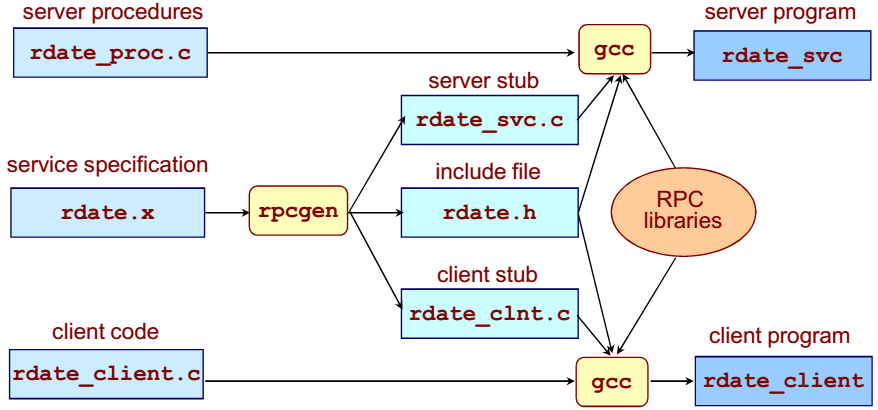
\includegraphics[width=0.7\linewidth]{img/sunrpc}
\caption{Funzionamento delle Sun RPC}
\label{fig:sunrpc}
\end{figure}
\begin{lstlisting}[language=IDL,caption="Esempio di file rdate.x",label=lst:rdate]
program RDATE_PROG {
    version RDATE_VERS {
        long BIN_DATE(void) = 1;	/* procedure number */
        string STR_DATE(long) = 2;	/* procedure number */
    } = 1;							/* version number   */
}= 0x20000001;						/* program number   */
\end{lstlisting}
Come detto il passaggio di parametri è consentito solo tramite copia, per molti linguaggi questo non è un problema in quanto non è supportato nemmeno a livello di linguaggio in altri contesti tuttavia è possibile utilizzare delle chiamate per \emph{valore/risultato} al posto della chiamata per riferimento.
\subsection{Remote method invocation}
La \emph{Remote Method Invocation} (RMI) sfrutta la stessa idea della RPC ma si basa su costruzioni di programmazione differenti, lo scopo è quello di ottenere i vantaggi di una programmazione Object-Oriented solamente in un contesto distribuito. Un'importante differenza rispetto alle RPC è che nelle RMI è possibile il passaggio di oggetti per riferimento, questo richiede il mantenimento delle relazioni con gli alias. In molti casi le RMI sono sviluppate su un livello di RPC.\\
Nelle RPC l'IDL separa l'interfaccia dall'implementazione, questa separazione è alla base dei principi di programmazione OO, è naturale posizionare l'interfaccia di un oggetto su di un host e l'implementazione su di un altro.\\
\subsubsection{Java RMI}
JAva RMI è il più semplice tra i moderni sistemi ad oggetti distribuiti più diffusi, esso si concentra solamente sulle chiamate di metodi remote il resto dei servizi è fornito da altri componenti della famiglia Java, permette di effettuare il download delle classi, di avere dei proxies dinamici.\\
Il concetto di interfaccia Java assume un nuovo ruolo con la distribuzione, un \emph{oggetto remoto} deve implementare un'interfaccia che estende \texttt{java.rmi.Remote} come nell'esempio del Listato \ref{lst:extendsRemote}
\begin{lstlisting}[language=Java,caption="Esempio di interfaccia remota",label=lst:extendsRemote]
import java.rmi.*
public interface AccountServer extends Remote {
	Account getAccount (int num) throws RemoteException;
}
\end{lstlisting}
Implementare un interfaccia remota non è sufficiente per accettare delle chiamate remote, per fare ciò è necessario \emph{esportare} l'oggetto.
Questo può essere fatto automaticamente nel costruttore se la classe deriva da \texttt{java.rmi.server.RemoteObject} come nel caso di \texttt{UnicastRemoteObject} oppure staticamente invocando il metodo \texttt{UnicastRemoteObject.exportObject}.\\
Per ottenere un riferimento ad un oggetto remoto esistono due modi, attraverno il passaggio di parametri o come valore di ritorno oppure interrogando esplicitamente un servizio di \emph{lookup} denominato \texttt{rmiregistry}. In entrambi i casi il riferimento all'oggetto remoto contiene lo stub del client ovvero implementa l'interfaccia remota, istanzia il \texttt{RemoteStub}. Una volta acquisito il riferimento remoto esso è indistinguibile da uno locale.\\
RMI non maschera completamente la distribuzione, notiamo la presenza di eccezioni ed interfacce remote, questo è il risultato di una precisa scelta progettuale per distingure un interazione locale da una remota. RMI inoltre è uno strumento poco potente rispetto agli altri sistemi ad oggetti distribuiti, tuttavia altri componenti Java sono costruiti su di esso come JavaEE.
%\section{CORBA}\label{capitolo3}
L'acronimo \textbf{CORBA} significa \emph{Common Object Request Broker Architeture} ed è il cuore dell'\emph{Open Managment Architeture} (OMA) un prodotto sviluppato dall'\emph{Open Managment Group} (OMG).\\
L'OMA è definito come un \emph{open framework} per applicazioni Object-Oriented distribuite, esso aiuta l'interoperabilità e fornisce mappature per diversi linguaggi di programmazione. Questo framework permette la progettazione di applicazioni distribuite come un insieme di oggetti cooperanti. I diversi programmi interagiscono tra loro come fossero eseguiti su di una singola macchina, trascurando il linguaggio con i quali sono stati sviluppati e l'hardware sui quali sono eseguiti.\\
L'OMG è un organismo di standardizzazione, esso fornisce solamente le specifiche e non l'implementazione di CORBA.\\
L'OMA definisce un \emph{Interface Definition Language} per specificare le API degli oggetti CORBA in termini di interfacce ed operazione. Un esempio della struttura di un sistema CORBA è mostrato in \figurename"\ref{fig:orb}.
\begin{figure}
\centering
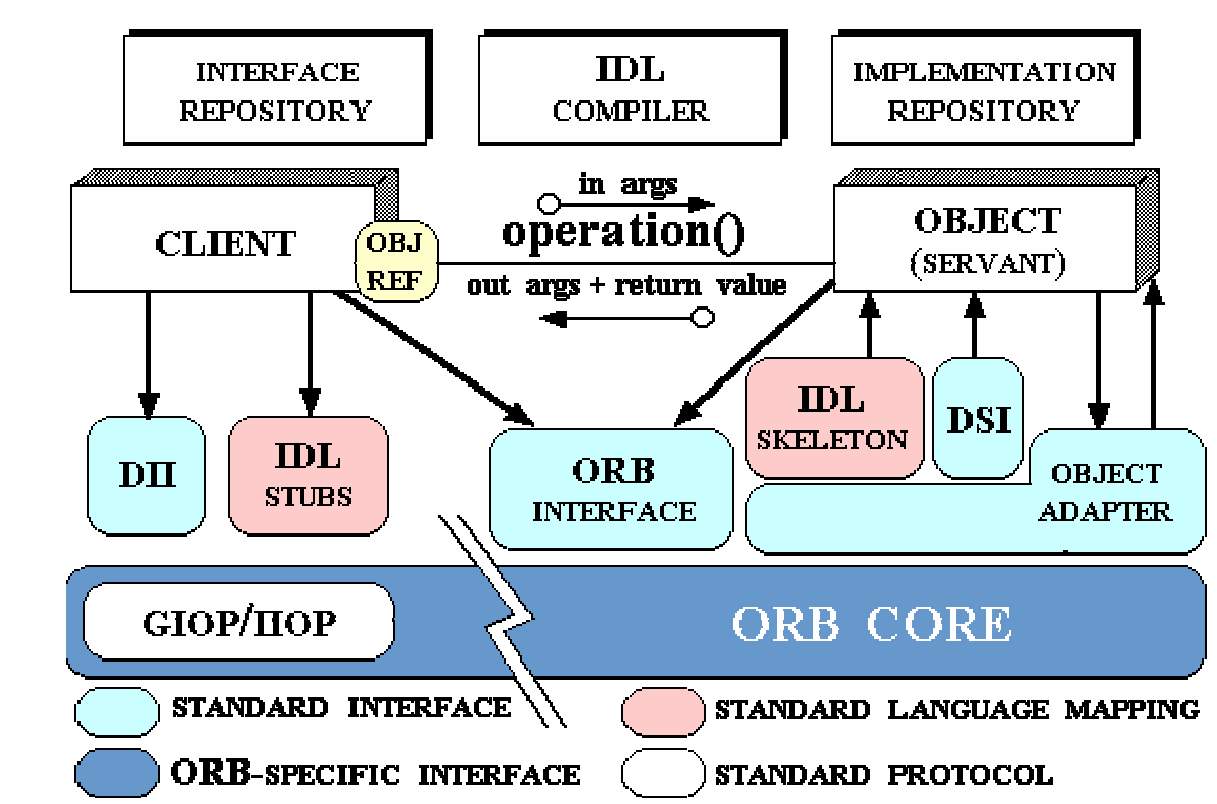
\includegraphics[width=0.7\linewidth]{img/orb}
\caption{Struttura di un sistema CORBA}
\label{fig:orb}
\end{figure}
L'\emph{Object Request Broker} è composto da diversi componenti, i principali sono il \emph{client}, il \emph{servant} e l'\emph{ORB Core}:
\begin{description}
	\item[Client:] è il componente che invoca i diversi servizi, esso mantiene un riferimento agli oggetti remoti.
	\item[Servant:] questo componente \emph{rappresenta} un oggetto CORBA, esso non è un vero e proprio oggetto in quanto gli oggetti CORBA sono solamente un concetto mentre un \emph{servant} è un oggetto nel linguaggio target che viene utilizzato per implementare uno o più oggetti CORBA. Quando un processo server riparte esso crea un nuovo \emph{servant} per rappresentare lo stesso oggetto CORBA.
	\item[ORB Core:] è responsabile dello smistamento e dell'inoltro delle chiamate agli oggetti remoti nascondendo così la comunicazione al programmatore. Il suo compito è quello di localizzare gli oggetti remoti, comunicare le richieste a questi oggetti, attendere un risultato ed infine restituire il risultato a chi lo ha richiesto.
	\item[ORB Interface:] è l'interfaccia standard per accedere ad un servizio del core, questo disaccoppia client e server da una specifica implementazione dell'ORB.
	\item[IDL Stub e Skeleton:] costruito dalle interfacce degli oggerri remoti tramite il compilatore IDL, insieme all'ORB permette il dispacciamento delle richieste al giusto oggetto remoto.
	\item[Dynamic Invokation Interface:] (DII) interfaccia standard utilizzata dal client per accedere ai servizi forniti da un oggetto remoto la cui interfaccia non era conosciuta a tempo di compilazione.
	\item[Dynamic Skeleton Interface:] (DSI) interfaccia standard utilizzata per implementare un oggetto remoto.
	\item[Object Adapter:] è il componente che gestisce la comunicazione tra l'oggetto remoto e l'ORB, esso incorpora i meccanismi e le policies principali per implementare le seguenti operazioni:
	\begin{itemize}
		\item Registrare, attivare e disattivare i servant
		\item Creare e interpretare i riferimenti agli oggetti
		\item mediare l'invocazione dei servizi
	\end{itemize}
	\item[GIOP e IIOP:] sono i protocolli utilizzati per connettere il client e il server sono standardizzati dal OMG.
\end{description}
Il \emph{Portable Object Adapter} (POA) come abbiamo visto, è un componente situato tra l'ORB e i servant, il client effettua una richiesta utilizzando un riferimento all'oggetto remoto, la richiesta viene ricevuta dall'ORB che inoltra la richiesta al POA che ospita l'oggetto. Il POA dispaccia la richiesta al servant di competenza il quale esegue l'operazione e restituisce il risultato al POA che a sua volta la inoltra all'ORB che la restituisce al client. Il POA deve soddisfare tre requisiti:
\begin{itemize}
	\item creare riferimenti agli oggetti per permettere al client di raggiungere l'oggetto remoto.
	\item assicurarsi che ogni oggetto target sia riferito ad un servant.
	\item ricevere le richieste dal parte client dell'ORB e indirizzarle verso il servant adatto.
\end{itemize}
Oltre alla parte principale di CORBA esistono una serie di servizi che forniscono una serie di funzionalità a supporto dell'integrazione e dell'interoperabilità degli oggetti distribuiti. Questi oggetti sono chiamati \emph{CORBA SErvice} o \emph{Object Service} e sono definiti come standard in CORBA da interfacce specificate in IDL. I principali servizi sono il servizio di \emph{Naming} e di \emph{Trading Object} che permettono al server di esporre i suoi servant. I servizi \emph{Event} e \emph{Notification} supportano la comunicazione asincrona multipla, il servizio \emph{Transaction} fornisce un supporta ai sistemi transazionali.\\
Il sistema CORBA, infine, fornisce delle \emph{horizontal facilities} e delle \emph{vertical facilities}, le prime si posizionano tra il middleware CORBA e i potenziali servizi utilizzati nel dominio di applicazione come una \emph{printing facility} o una \emph{mobile agent facility}.
Le \emph{Vertical Facilities} definiscono delle interfacce standard per quegli oggetti che ogni settore del dominio vuole condividere.
\subsection{CORBA e Java}
Java include di default un'implementazione base, ma completamente funzionante di CORBA, un IDL per il compilatore Java e un Naming Service.\\
Lo scopo dell'IDL è quello di permettere la definizione delle interfacce degli oggetti in un modo indipendente dal linguaggio di programmazione utilizzato per l'implementazione. Per chiamare una funzione di un oggetto CORBA tutto quello che è necessario al client è l'IDL dell'oggetto. l'IDL supporta \emph{multiple inheritance} e \emph{genericity}, esso supporta parametri sia in input che in output sia bidirezionali, le operazioni possono sollevare delle \emph{eccezioni} definite nell'IDL, infine, esso fornisce una serie di tipi di dato come \texttt{string, boolean, int, long, float} e \texttt{double} ma permette anche la definizione di tipi complessi tramite \texttt{struct, sequence, array, typedef, enum} e \texttt{union}.
Un esempio di file IDL è quello del Listato \ref{lst:idlexemp}
\lstinputlisting[language=IDL,caption="Esempio di file IDL",label=lst:idlexemp]{listati/account.idl}
Per un'analisi approfondita sullo sviluppo di una applicazione con CORBA si rimanda a \cite{cugola:corba} e \cite{sun:corba}
%\section{Programmazione concorrente con OpenMP}\label{capitolo4}
OpenMP è una API multi-piattaforma per il calcolo parallelo a memoria condivisa, essa è disponibile per tutti i sistemi operativi e per i linguaggi C/C++ e Fortran. Questa API si basa su direttive del compilatore, routine di librerie e variabili d'ambiente.\\
Più in dettaglio OpenMP è un'implementazione del multi-threading, nel quale un processo \emph{master} effettua una \emph{fork} e genera un determinato numero di thread \emph{slave} sul quale suddividere il lavoro. Questi thread slave vengono eseguiti concorrentemente su differenti core o processori come mostrato in \ref{fig:openmp}.\\
\begin{figure}
\centering
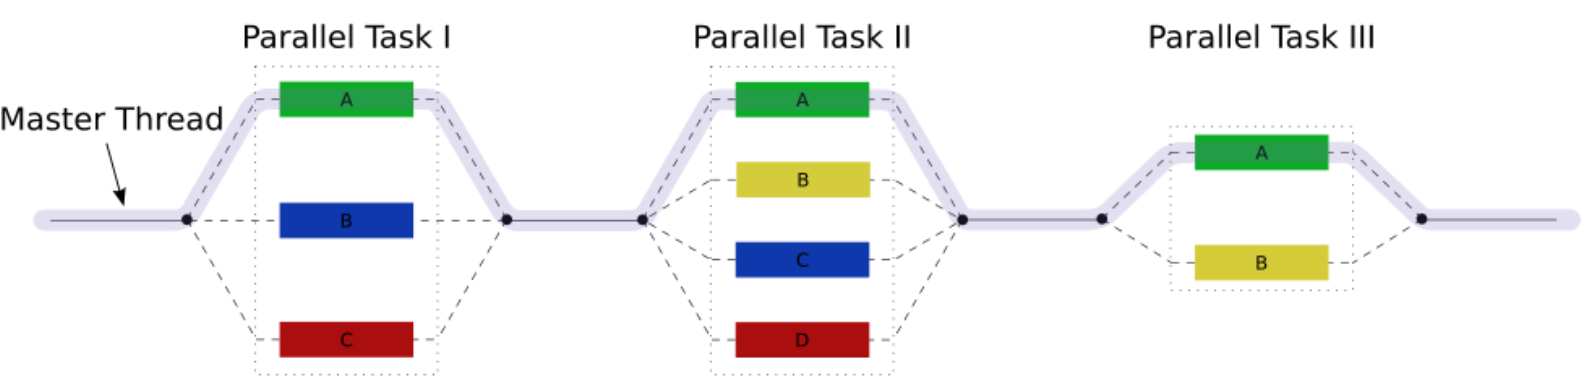
\includegraphics[width=0.7\linewidth]{img/openmp}
\caption{Suddivisione del carico tra diversi threads}
\label{fig:openmp}
\end{figure}
La maggior parte dei costrutti di OpenMP sono direttive del compilatore o \texttt{pragmas}, lo scopo principale dei questa API è quello di parallelizzare i cicli e per farlo offre un approccio incrementale al parallelismo.
Alcune peculiarità sono:
\begin{itemize}
	\item \textbf{Parallelismo innestato:} le API permettono di costruire del thread all'interno di altri thread.
	\item \textbf{Dynamic thread:} le API permettono di cambiare dinamicamente il numero di thread in esecuzione nelle differenti aree parallelizzate.
	\item \textbf{Input/Output: OpenMP} non specifica nulla riguardo agli I/O paralleli è compito del programmatore perciò assicurare la corretta esecuzione parallela.
	\item \textbf{Memory Consistency:} i threads mantengono una loro \emph{cache} e non è quindi necessario mantenere una consistenza con la memoria principale, tuttavia in caso di una variabile condivisa è responsabilità del programmatore assicurare il corretto uso della variabile.
\end{itemize}
Vediamo ora nel Listato \ref{lst:helloopen} un esempio di utilizzo delle API OpenMP
\begin{lstlisting}[language=C++,caption={Esempio di utilizzo delle OpenMP},label=lst:helloopen]
#include <omp.h>
#include <iostream>

using namespace std;
int main () {
	#pragma omp parallel num_threads(3)
	{
		cout<<"Hello World\n"
	}	
}
\end{lstlisting}
Per compilare tale codice è necessario aggiungere l'opzione \texttt{-fopenmp} al normale comando di compilazione.\\
Le direttive OpenMP valide sono identificate dal costrutto
\begin{verbatim}
		#pragma omp name [clause, ...]
\end{verbatim}
dove \emph{name} identifica la direttiva la quale può essere seguita da una o più opzioni. Una delle direttive più importanti è la direttiva \texttt{parallel} senza la quale un programma verrebbe eseguito sequenzialmente. Quando un thread raggiunge la direttiva \texttt{parallel} esso crea una team di  threads ed esso ne diventa il master. A partire dall'inizio della regione parallela il codice viene duplicato e tutti i thread eseguono lo stesso codice. Esiste un \emph{barrier} implicito alla fine della regione parallela dopo il quale solo il thread master continua l'esecuzione.
Se un thread termina all'interno di una regione parallela tutti i thread del team terminano ed l'esecuzione da quel punto è indefinita.
%\section{Advance message passing with MPI}\label{capitolo5}
Il \emph{Message PAssin Interface} (MPI) è un middlewaare studiato per il calcolo ad alte performance; in realtà MPI è solo uno standard che specifica una API esistono poi diverse implementazioni, la più diffusa forse è \emph{OpenMPI}.\\
Lo scopo di MPI era quello di sviluppare uno standard per un API per il calcolo distribuito ad alte prestazioni che fosse facile da utilizzare, portabile, efficiente e flessibile.\\
Le chiamate a funzioni sono molto semplice e hanno una struttura del tipo
\begin{verbatim}
	rc = MPI_Xxxx (parameter,...)}
\end{verbatim}
dove \texttt{rc} restituisce il codice \texttt{MPI\_SUCCESS} in caso di esecuzione corretta del comando. Un esempio di codice MPI è mostrato nel listato \ref{lst:mpihello}
\begin{lstlisting}[language=C,caption={Hello World con MPI},label=lst:mpihello]
#include "mpi.h"
#include <stdio.h>

int main (int argc, char *arrgv[]) {
	MPI_Init (&argc,&argv);
	printf("Hello world!\n");
	MPI_Finalize();
	return 0
}
\end{lstlisting}
MPI utilizza degli oggetti chiamati \emph{comunicators} e \emph{groups} per organizare delle collezioni di processi e definire lo scopo della comunicazione. Molte delle routine MPI richiedono di specificare un comunicatore come argomento, il comunicatore predefinito è \texttt{MPI\_COMM\_WORLD} ed include tutti i processi MPI. Insieme ad un comunicatore ad ogni processo viene assegnato un proprio \emph{rank}, ovvero un ID univoco che parte da $ 0 $ ed è incrementato progressivamente, questo rank permettte al programmatore di specificare la sorgente e la destinazione di un messaggio ma anche per controllare il flusso di esecuzione.\\
L'API MPI fornisce una serie di funzioni per controllare ed interrogare l'ambente:
\begin{itemize}
	\item \texttt{int MPI\_Comm\_size(MPI\_Comm\_comm, int *size)} serve per reperire il numero di processi presenti in uno specifico comunicatore.
	\item \texttt{int MPI\_Comm\_rank(MPI\_Comm\_comm, int * rank)} restituisce il rank del processo MPI chiamante all'interno del comunicatore specificato.
	\item \texttt{int MPI\_Get\_processor\_name (char *name, int *resultlen)} restituisce il nome del processo chiamante tuttavia questa funzione è dipendente dall'implementazione.
\end{itemize}
La maggior parte delle routine MPI può essere utilizzata sia in modalità bloccante che non bloccante, nel caso di comunicazione bloccante la \emph{send} restituisce il controllo al programma solo dopo che il buffer è stato svuotato ed è quindi modificabile, questo tuttavia non comporta che i dati siano stati ricevuti, solo nel caso di comunicazione sincrona, e quindi di risposta del ricevente si ha questa certezza; la \emph{receive} invece restituisce il controllo al programma solo quando tutti i dati sono arrivati e sono pronti per essere utilizzati. Nel caso di chiamate non bloccanti sia la \emph{send} che la \emph{receive} non attendono la comunicazione è perciò pericoloso modificare il buffer fino a quando non si è certi che la comunicazione non è stata effettuata. MPI inoltre garantisce l'ordinamento dei messaggi in un singolo processo tuttavia nel caso di multi-threading non si può controllare quale sia il messaggio ricevuto per primo.\\
La nostra trattazione non si spingerà oltre in quanto le slide \cite{cugola:mpi} trattano argomenti più tecnici che teorici e che quindi verrebberò riportati tali e quali. Oltre alle slide già citate si rimanda anche al tutorial su internet \cite{tutorial:mpi}
%\section{Message oriented middleware}\label{capitolo6}
RPC e RMI favoriscono un modello di comunicazione di tipo sincrono il quale è un'astrazione più naturale per il programmatore, tuttavia esso supporta solamente interazioni \emph{punto-punto}, inoltre risulta essere molto costoso e richiede un forte accoppiamento tra chiamante e chiamato.\\
Il sistema di comunicazione \emph{asincrono} si incentra sulla nozione di \emph{evento/messaggio}, essa supporta la comunicazione multi-punto e quindi permette un disaccoppiamento tra i componenti. La forma di comunicazione asincrona più diffusa è quella basata sullo scambio dei messaggi, tipicamente gestita direttamente o magari fornita da funzionalità di rete del sistema operativo. Esistono poi dei \emph{Middleware Orientati ai Messaggi} (MOM) che forniscono un'infrastruttura a livello applicativo tra diversi \emph{comunication server}.\\
I MOM forniscono sia comunicazione di tipo sincrono che asincrono, ma l'aspetto fondamentale è che i MOM sono in grado di fornire oltre alla comunicazione di tipo \emph{transiente} nel quale \emph{sender} e \emph{recipients} sono in esecuzione al momento della comunicazione, anche comunicazione di tipo \emph{persistente} nella quale i messaggi vengono immagazzinati dal sistema fino a quando non possono essere recapitati. Esistono due tipologie principali nelle comunicazioni \emph{message oriented}, la prima è la \emph{message queuing} la seconda è il modello \emph{publish-subscribe}; entrambe le tipologie sono orientate ai messaggi, offrono un forte disaccoppiamento tra componenti ed entrambe si basano su di una serie di server per instradare i messaggi e supportare la persistenza.\\
Tuttavia il \emph{message queuing} prevede un tipo di comunicazione punto-punto asincrona e persistente, essa garantisce sempre che il messaggio venga inserito nella coda del destinatario ma non garantisce nulla sul suo comportamento, il sistema risulta perciò disaccoppiato nel tempo e nello spazio e può essere visto come una generalizzazione delle e-mail.
Il sistema risulta essere intrinsecamente peer-to-peer, ogni componente mantiene una coda di input e una di output.
La comunicazione tramite code di messaggi può semplificare anche la comunicazione client server, il client inserisce una richiesta nella coda del server, il server in modo asincrono preleva tale richiesta la processa e restituisce il risultato nella coda del client. Tale meccanismo permette al client di disconnettersi dopo l'invio della richiesta e proseguire nella sua esecuzione, inoltre l'utilizzo delle code permette di semplificare il bilanciamento del carico come si vede in \figurename"\ref{fig:messagequeue}.
\begin{figure}
\centering
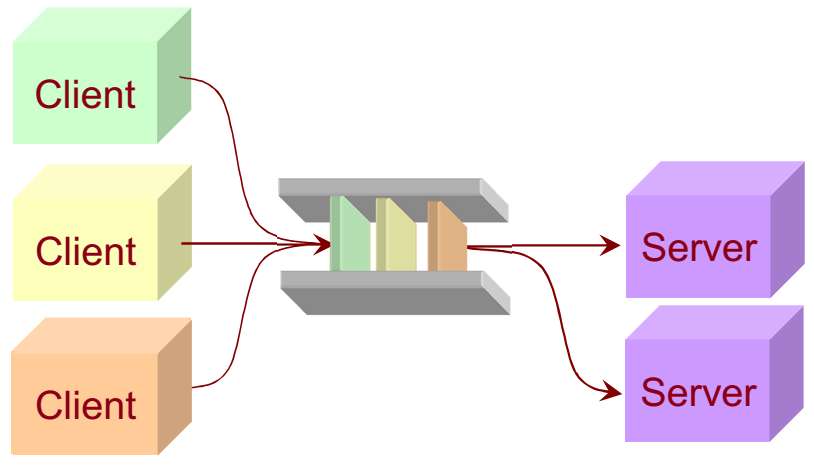
\includegraphics[width=0.7\linewidth]{img/messagequeue}
\caption{Sistema client server basato sulle code di messaggi}
\label{fig:messagequeue}
\end{figure}
Le code sono identificate da nomi simbolici è perciò necessario fornire un servizio di lookup, le code sono gestite da un \emph{queue managers} che può essere locale o remoto.\\
Nella comunicazione \emph{publish-subscribe} i componenti dell'applicazione pubblicano in modo asincrono delle \emph{notifiche}, queste notifiche solitamente sono generate in reazione al verificarsi di un \emph{evento}. I componenti possono dichiarare il loro interesse rispetto a particolari eventi utilizzando un meccanismo di \emph{sottoscrizione}; tali sottoscrizioni sono raccolte da un \emph{event dispatcher} il quale si occupa anche di instradare le notifiche ai diversi sottoscrittori. In base all'espressività del linguaggio di sottoscrizione è possibile distinguere due meccanismi:
\begin{description}
	\item[\emph{Subject-based:}] in questo caso ci si può sottoscrivere ad un insieme ristretto di eventi i cui argomenti sono determinati a priori.
	\item[\emph{Content-based:}] la sottoscrizione contiene un espressione che permette all'event dispatcher di filtrare i messaggi in base al loro contenuto.
\end{description}
\subsection{JMS}
La \emph{Java Message Service} è un API che permette la creazione l'invio, la ricezione  e la lettura dei messaggi all'interno di un sistema enterprise. JMS fornisce tre concetti principali:
\begin{itemize}
	\item \emph{JMS provider:} è l'entità che implementa l'API per la produzione di messaggi
	\item \emph{JMS Client:} è l'applicativo che sfrutta il servizio fornito dal JMS provider.
	\item \emph{JMS domains:} fornisce l'ambiente point-tp-point o publish-subscribe.
\end{itemize}
In JMS esistono dei domini per ogni tipo di comunicazione sia quello point-to-point nel quale ogni messaggio è indirizzato ad una coda specifica e i client estraggono i messaggi da code prestabilite per mantenere i loro messaggi. Il domino di comunicazione publish-subscribe invece è centrato su una gerarchia di topic, JMS, infine mette a disposizione una serie di interfacce indipendenti dal dominio che permettono la comunicazione in entrambi i domini, queste interfacce vengono chiamate \emph{common interface}.\\
Per una trattazione completa si rimandano alle slide dell'insegnante \cite{cugola:jms} un altro tutorial è quello messo a disposizione da Oracle \cite{sun:jms}, infine un implementazione Open Source di jms è JORAM \cite{joram:jms}.

%\section{Hadoop}\label{capitolo7}
Al giorno d'oggi produciamo dati ad una velocità impressionante, gli archivi di internet crescono di 20TB al mese, 100TB di dati sono caricati su Facebook ogni giorno. Insieme ai dati di internet crescono anche quelli personali e quelli prodotti dalle macchine.\\
Volendo analizzare questi dati tuttavia si incorrono in diversi problemi, il principale è che le capacità e le velocità dei dischi non sono migliorate di molto negli ultimi anni, tuttavia una soluzione è quella di parallelizzare gli \emph{storage} ma questo comporta problemi di aggregazione dei dati e di replicazione hardware.
Una soluzione a questi problemi potrebbe essere \emph{Hadoop} un sistema di distribuzione dei file che implementa anche un analisi dei dati tramite \emph{map reduce}. A differenza di database relazionali Hadoop non lavora soffre delle latenze dei dischi e non necessita di dati strutturati per lavorare con efficienza, inoltre, il MapReduce scala in maniera lineare. Rispetto al \emph{Volunteer computing} che lavora tramite rete Internet con computer dei quali non si può verificarne l'affidabilità, Hadoop lavora in un cluster locale sfruttando reti ad alte performance.\\
\subsection{La storia}
Nel 2002 Mike Cafarella e Doug Cutting iniziano a lavorare su \emph{Apache Nutch} un nuovo motore di ricerca. Nel 2003 Google pubblica un articolo sul \emph{Google File System} un filesystem distribuito e Mike e Doug iniziano a lavorare ad un progetto simile ma open source. Nel 2004 Google pubblica un ulteriore articolo sul modello di computazione denominato \emph{MapReduce} e ancora una volta Mike e Doug ne implementano una versione open source in Nutch. Nel 2006 questi due progetti si separano da Nutch e diventano \emph{Hadoop}, nello stesso anno Dug inizia a lavorare per "Yahoo!" dove inizia ad usare Handoop. Nel 2008 Yahoo!, Last.fm, Facebook e NYT utilizzano Hadoop. Nel 2009 Yahoo! fa segnare un nuovo record mondiale ordinando 1TB di dati in 62 secondi. Da quel giorno Hadoop è diventato uno standard per l'industria.\\
\subsection{MapReduce}
Il \emph{MapReduce} è un medello per l'analisi di una grande quantità di dati, questi dati sono organizzati come un insieme \emph{chiave-valore}; questo modello si suddivide in due fasi
\begin{itemize}
	\item $map(k_1,v_1) \rightarrow list(k_2,v_2)$  nella quale il dominio di input è diverso dal dominio dell'output
	\item una fase intermedia serve a ordinare la mappa risultante e raggrupparla per chiavi
	\item $reduce(k_2,list(v_2))\rightarrow list(v_3)$ dove il dominio di input e di output coincidono
\end{itemize}
Prima di spiegare in dettaglio il funzionamento doppiamo introdurre alcune definizioni:
\begin{description}
	\item[Job:] è un unità di lavoro eseguita dal sistema che comprende
	\begin{itemize}
		\item dati di input
		\item implementazione del \emph{map} e del \emph{reduce}
		\item configurazione
	\end{itemize}
	\item[Map task e Reduce task:] piccoli frammenti di un job
	\item[Jobtracker:] nodo del cluster che coordina i lavori
	\item[Tasktracker:] esegue un task e restituice il risultato al jobtraker
	\item[Split:] frammento di input
\end{description}
Il jobtracker divide i dati di input in parti e per ogni split di dati viene eseguito un \emph{map task}. Questa esecuzione avviene in parallelo su tutti i nodi, hadoop tenta di eseguire il task di riduzione sulla macchina nel quale risiedono i dati. Il risultato viene scritto sul disco della macchina e non sul HDFS. Il \emph{reduce task} riceve i dati attraverso la rete ed infine il risultato è salvato sull HDFS. In \figurename"\ref{fig:mapreduce} vediamo un esempio di questo procedimento.
\begin{figure}
\centering
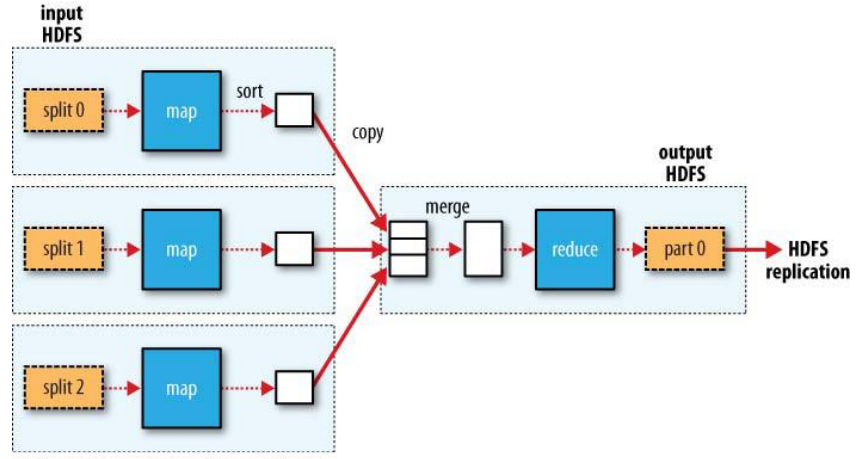
\includegraphics[width=0.7\linewidth]{img/mapreduce}
\caption{Esempio di MapReduce con Hadoop}
\label{fig:mapreduce}
\end{figure}
A volte si rende necessario effettuare delle operazioni sui dati intermedi, le possibile operazioni sono funzioni di combinazione che aggregano i dati per minimizzare il trasferimento sulla rete; e l'operazione di \emph{shuffle} ovvero un ordinamento dei dati di output.\\
In hadoop tutto è configurabile, il numero dei task sia di map che di reduce, la compressione dei dati, la gestione della memoria. Vengono creati dei profili per cercare di capire come migliorare le performance.\\
Per un esempio di come implementare un MapReduce in Hadoop si rimanda a \cite{cugola:hadoop}
\subsection{Hadoop Distributed File System}
\emph{Hadoop Distributed File System} (HDFS) è un filesystem appositamente progettato per lavorare con dati molto grandi ed adatto per accedere ai dati in streaming.
Dalla versione 2 di Hadoop HDFS è composto da un singolo \emph{namenode} (master) e una serie di \emph{datanode}(slave), il namenode gestisce il namespace del filesistem, esso mantiene l'immagine del namespase e scrive i file di log, esso ha inoltre una lista di tutti i datanode e delle informazioni in essi immagazzinate, tuttavia esso non mantiene alcun file.
I datanode sono macchine nelle quali vengono immagazzinati dei blocchi di file, essi comunicano continuamente con il namenode. Ogni file caricato sul HDFS è diviso in blocchi da 64MB in modo da minimizzare lo \emph{seek} e massimizzare il \emph{transfert rate}. Se un blocco è più piccolo di 64MB esso, a differenza di un normale filesystem, non occupa 64MB. Un file potrebbe essere più grande di un singolo disco in rete.\\
Mappers e Reducer utilizzano dei particolari tipi di dato che sono definiti da Hadoop e sono di tipo \emph{wrapping} ovvero ottimizzati per la serializzazione su rete. Per aggiungere nuovi tipi di dato bisogna implementare le due interfacce \texttt{Writeable} e \texttt{WriteableComparable}.
\subsection{PIG}
Pig è un linguaggio che permette l'interrogazione complessa di dati riccamente strutturati. Uno script è una sequenza di trasformazioni sui dati iniziali che può essere tradotta in un \emph{MapReduce job}, è veloce da sviluppare, può essere scritta in poche righe ed eseguita su terabytes di dati.\\
Pig può essere eseguito in tre modi, tramite script, tramite \emph{interactive shell}, oppure embeddato in Java.
\subsection{Approfondimenti}
Per eventuali approfondimenti e alcuni esempi si rimanda alle slide del corso \cite{cugola:hadoop}. Per l'installazione e i tutorial si rimandano alle pagine ufficiali di Hadoop \cite{hadoop:docs} \cite{hadoop:tutorials}
%\section{Programming WSNs with TinyOS}\label{capitolo8}
\subsection{Wireless Sensor Networks}
Le WSN sono reti di sensori che si contraddistinguono dalle normali reti per il gran numero di nodi presenti ma molto densi, questi nodi solitamente non hanno un ID globale come un IP. Le WSN non sono interattiva ma si basano su applicazioni data-centriche e evento-centriche. La comunicazione è di tipo asimmetrica dai nodi verso un datacenter centrale, molto spesso la comunicazione è \emph{content-based} rispetto a una comunicazione \emph{identity-based}. Il tipo di rete utilizzata dipende molto dall'applicazione. Solitamente questo tipo di reti sono sviluppate e installate in ambienti ostili e inaccessibili, per questo i sensori devono auto-organizzarsi, essere \emph{exception-free} ovvero non presentare comportamenti indesiderati e soprattutto è impossibile sostituire la fonte di energia perciò è necessario che l'utilizzo di tale risorsa sia gestito accuratamente.\\
Nella maggior parte dei casi i sensori sono fissi e molto ravvicinati, tuttavia esistono casi in cui questo non è vero come nel caso di applicazioni mobile come nei body sensor network; in ogni caso abbiamo che i sensori sono fissi è solo l'ambiente in cui sono posizionati che si muove.\\
Come nelle comunicazioni mobili standard anche in questo caso che la comunicazione è il punto centrale del sistema ed è necessario sfruttare al massimo la comunicazione wireless tenendo conto di tutti i problemi derivanti come collisioni, effetti mulitpath ecc.; inoltre la comunicazione è l'attività che consuma più energia, la banda è scarsa e deve essere condivisa, infine, la topologia è dinamica. Tuttavia esistono diverse differenze rispetto ad una rete wireless tradizionale, innanzi tutto il numero dei nodi è molto maggiore è quindi impossibile identificarli tramite un ID globale, il fattore energetico è molto più restrittivo, la natura della comunicazione è diversa ma soprattutto i nodi di una rete tradizionali sono indipendenti gli uni dagli altri nelle WSN questo non è possibile.\\
Un altro dispositivo simile ad un sensore di una WSN è RFID (\emph{Radio Frequency Identification}) il quale viene utilizzato in moltissime applicazioni come ad esempio al posto delle chiavi o dei codici a barre. Un sensore RFID è simile ad un sensore di una WSN in quanto entrambi interagiscono con l'ambiente, ed entrambi utilizzano il wireless per la comunicazione. Tuttavia RFID è un dispositivo passivo ovvero non ha bisogno di energia per funzionare, ed inoltre sono dispositivi stupidi non in grado di effettuare alcuna computazione.\\
Le applicazioni nelle quali si utilizzano WSN sono i più vari, partiamo da ambiti militari dove si utilizzano per monitorare gli equipaggiamenti, le munizioni, le forze alleate ma anche come identificazione di attacchi nucleari biologici o chimici. Si utilizzano inoltre come applicazioni per monitorare l'ambiente sia come semplici sensori per le condizioni ambientali a monitoraggi più complessi come monitoraggi di terreno e piante o anche monitoraggi di frane ed incendi forestali. In ambito medicale si possono monitorare la posizione di dottori e pazienti all'interno di un ospedale, la somministrazione dei medicinali, telemonitoring di dati fisiologici nei pazienti.
\subsection{Architettura della comunicazione}
La comunicazione è alla base di una WSN, esiste una grande varietà di combinazioni tra i diversi livelli di comunicazione per combinare ad esempio un efficente consumo di energia per la comunicazione tramite il mezzo wireless. Si cerca perciò di favorire l'interoperabilità.\\
Ma perchè non utilizzare i normali protocolli di routing? I motivi sono molti ad esempio l'impossibilità di utilizzare un identificativo per i nodi univoco a causa dell'alto numero di nodi, inoltre i sensori sono molto limitati in consumi, potenza di calcolo e memoria; sono sottoposti ad un alta probabilità di fallimento ed infine la topologia cambia frequentemente.\\
Esistono diversi protocolli di routing che si possono suddividere in diverse categorie:
\begin{itemize}
	\item Protocolli data-centrici: flooding, gossiping, SPIN, SAR, ecc.
	\item Protocolli gerarchici: LEACH , TEEN, APTEEN, PEGASIS
	\item Protocolli basati sulla posizione: MECN, SMECN, GEAR
\end{itemize}
\subsubsection{Routing data centrico}
Da quando i sensori vengono posizionati in gran numero ed in modo casuale è difficile assegnargli degli §§ID specifici e senza un identificativo univoco è quasi impossibile prelevare i dati; tuttavia esiste una soluzione per prelevare e dirigere i dati verso il centro di raccolta, questo tipo di protocolli si basano sulla descrizione dei dati. Tuttavia questo richiede che i dati siano corredati da attributi nominati in modo che essi possano essere interrogati facilmente.\\
Alcuni algoritmi si basano sulla disseminazione dei dati come il \emph{Flooding} che invia i dati a tutti i vicini e il \emph{Gossiping} che invia i dati ad un vicino selezionato casualmente, entrambi questi algoritmi sono semplici ma portano ad un implosione in quanto molti dati raggiungono uno stesso nodo ed inoltre vi è una sovrapposizione in quanto più nodi possono leggere gli stessi valori ma soprattutto questi due protocolli sono inefficienti a livello di consumo di energia.\\
Esistono poi degli algoritmi di \emph{diffusione diretta} in questo caso ogni sensore assegna degli attributi ad ogni dato generato, gli altri nodi esprimono il loro \emph{interesse} verso alcuni di questi attributi, questo interesse può essere quantificato da un \emph{gradiente} che indirizza la diffusione dei dati. La consegna dei dati segue la strada imposta dal gradiente, tale meccanismo è simile al content-based nel contesto del publish-subscribe. Uno dei protocolli che sfrutta questo fattore è il \emph{CCBR (Context and Context Based Routing)} in questo caso l'interazione tra i nodi è di tipo datacentrica ma anche di tipo \emph{context aware}. In questo protocollo ogni nodo mantiene traccia dalla distanza che lo separa dal collettore dei dati, le proprietà dei nodi sono mantenute dai nodi stessi e il content based è effettuato solo dai nodi che inviano i dati. Il CCBR sfrutta alcune caratteristiche:
\begin{itemize}
	\item utilizza \emph{link-layer brodcast} quando è possibile per essere robusto contro il cambio di topologia e minimizzare il traffico
	\item usa un approccio \emph{receiver-based} ovvero è il nodo ricevente che decide se accettare il pacchetto in ingresso e reinviarlo.
	\item si utilizza un approccio \emph{opportunistico} ogni nodo decide se inoltrare il pacchetto in base ad una decisione locale la quale dipende dalla sua distanza dal centro di raccolta.
	\item infine si utilizza un meccanismo di \emph{ack implicito}
\end{itemize}
\subsubsection{Protocollo gerarchico}
I protocolli di tipo gerarchico sono stati introdotti perché sono più efficienti sia in termini di overhead di traffico sia in termini di consumo di energia, i diversi sensori formano un cluster che viene controllato da una \emph{cluster-head} la quale aggrega e fonde i dati per risparmiare energia.\\
Uno dei più diffusi protocolli gerarchici è il \emph{LEACH (Low Energy Adaptative Clustering Hierarchy)} il quale sfrutta l'idea di selezionare in modo casuale la testa del cluster e questa può utilizzare uno qualsiasi dei protocolli di route affidabili per inviare dati al sink. L'algoritmo si suddivide in due fasi che vengono ripetute periodicamente la prima fase detta di \emph{setup} comporta che un insieme di nodi a caso elegga se stesso come testa del cluster, questi nodi avvisano tutti gli altri di essere la testa, gli altri nodi selezionano la testa in base al valore RSSI (risparmio di energia). La seconda fase è chiamata di \emph{steady state} durante questa fase i sensori raccolgono i dati e le inviano all'head la quale li raccoglie e li aggrega.
%\include{capitolo9}
\end{document}